\documentclass[12pt, titlepage, oneside]{article}
\usepackage[letterpaper, margin=1in]{geometry}
\usepackage{siunitx, booktabs, amsmath, enumitem, pdfpages, tabularx,caption, graphicx, pgfplots, textcomp}
\usepackage[siunitx]{circuitikz}
\sisetup{detect-weight=true, detect-family=true}
\usepackage{wrapfig}
\usepackage{mathrsfs}
\setlength\parindent{0pt}
\let\oldhat\hat
\let\oldvec\vec
\newcommand{\cross}{\bm{\times}}
\renewcommand{\hat}[1]{\oldhat{\mathbf{#1}}}
\usepackage{bm}
\renewcommand{\vec}[1]{\oldvec{\bm{#1}}}
\renewcommand{\hat}[1]{\oldhat{\bm{#1}}}
\renewcommand{\b}[1]{\textbf{#1}}

\begin{document}
\section*{28.1 Electromotive Force}

\textbf{Direct Current} is the type of current a typical battery would deliver.\\

The \textbf{emf $\mathscr{E}$} is the maximum voltage a battery can provide between its terminals.
\\

Note to self: The idea of saying "current flow" is incorrect. Since current is the flow of charge, current flow would imply you are talking about the flow of flow of charge.
\\

\begin{wrapfigure}{r}{0.3\textwidth}
	\begin{center}
		\vspace{-1.5cm}
		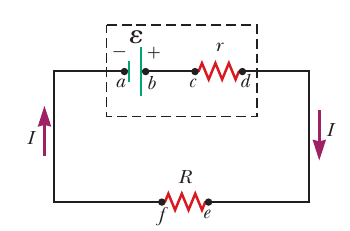
\includegraphics[scale=0.5]{1.png}
	\end{center}
\end{wrapfigure}
For a theoretical battery, the voltage across the terminals would be equal to its emf. But in reality, there exists some resistance due to batteries consist of matter, and there is resistance to the flow of charge.
\\

 A battery can be thought of as a theoretical battery $\mathscr{E}$ in series with a resistor of value $r$, where $r$ is the internal resistance of the material.
 \\
 
 We are able to see now that the real voltage of the battery due to the internal resistance voltage drop is,
 \begin{align*}
 	\Delta V = \mathscr{E} - Ir
 \end{align*}
Notice that $ \mathscr{E} $ only is at its true value when in an open circuit.
\\

The resistor $R$ in the figure above is known as the load resistance. With this load resistor, we can solve for the emf.\\

\noindent\fbox{%
	\parbox{\textwidth}{%
		\textbf{EMF}
\begin{align}
\mathscr{E} = Ir + IR
\end{align}
}}\\

Solving for $ I  $ yield,
\begin{align*}
	I = \frac{\mathscr{E}}{R+r}
\end{align*}
Notice that multiplying equation 1 by $ I $ provides the total power,\\

\noindent\fbox{%
	\parbox{\textwidth}{%
		\textbf{Total Power}
\begin{align}
	I\mathscr{E} = I^2R + I^2r = P_R + P_r
\end{align}
}}
\newpage
Ex. Find the load resistance for the maximum power.
\begin{align*}
P = I^2R = \frac{\mathscr{E}^2R}{(R+r)^2}
\end{align*}
Maximize R using Calculus 1 techniques, 
\begin{align*}
&\frac{dP}{dR} = \frac{d}{dR} \Bigg[\frac{\mathscr{E}^2R}{(R+r)^2}\Bigg] = [\mathscr{E}^2(R+r)^{-2}] + [\mathscr{E}^2R(-2)(R+r)^{-3}]=0\\
&\dfrac{\mathscr{E}^2(R+r)}{(R+r)^3} - \dfrac{2 \mathscr{E}^2R}{(R+r)^3} = \dfrac{\mathscr{E}^2(r-R)}{(R+r)^3} = 0\\
&\frac{\mathscr{E}^2(r-R)}{(R+r)^3} = 0
\end{align*}
Solve for R
\begin{align*}
R=r
\end{align*}
Therefore for max power delivery, we require the load voltage equal to the internal resistance.\\

From this we can also inspect a very important idea. To calculate the max power, we can calculate the max power that can be delivered to the circuit.

\begin{align*}
P_{max} = \frac{\mathscr{E}^2}{4R^2}
\end{align*}
\section*{28.2 Resistors in Parallel or Series}

Since current is the rate of charge through an area inside the circuit. Therefore, in a series combination, the current should be the same throughout as the same charges pass through every component in the circuit.\\

\noindent\fbox{%
	\parbox{\textwidth}{%
		\textbf{Current in Series}
		\begin{align}
		I = I_1 = I_1 = ... = I_n
		\end{align}
		 Current through a series circuit is the same throughout.
		}}\\
	
	Since we know that the total potential difference is the sum of the voltage drops in the circuit,
	\begin{align*}
	\Delta V = \Delta V_1 + \Delta V_2 + ... + \Delta V_n
	\end{align*}
	We can rewrite this as,
	\begin{align*}
	\Delta V = IR_1 + IR_2 + ... + IR_n
	\end{align*}	
	\noindent\fbox{%
		\parbox{\textwidth}{%
			\textbf{Resistors in Series}
			\begin{align}
			\Delta V = IR_{eq}
			\end{align}
			Where $R_{eq} = R_1 + R_2 + ... + R_n$ 
		}}
		\begin{center}
			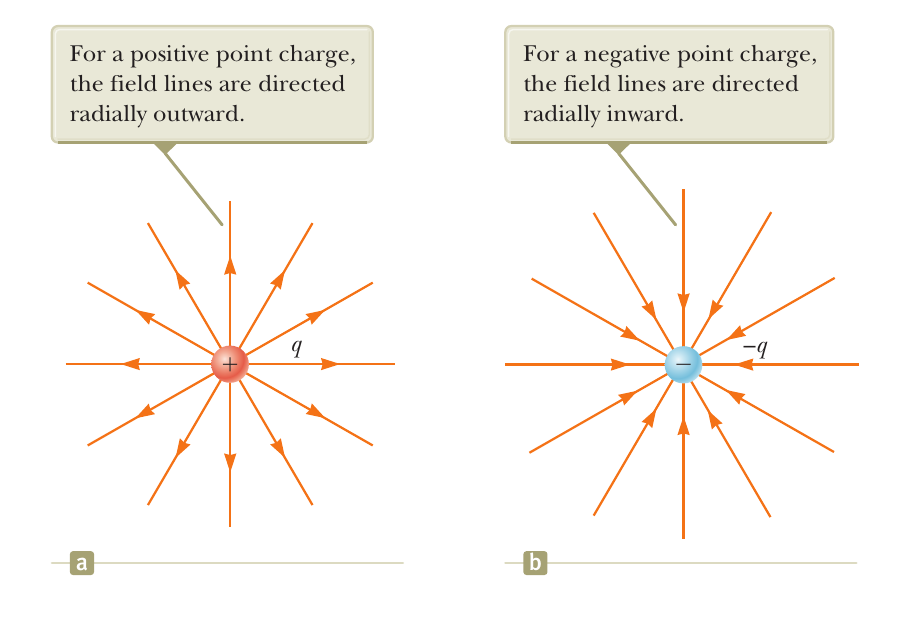
\includegraphics[scale=0.4]{2.png} Simple Series Circuit
		\end{center}
	In parallel, we understand there is a $\Delta V$ across the terminals of the battery, but if there was resistors also across the terminal, all the resistors would have the same drop as they are all connected to the same node.\\
	

			\noindent\fbox{%
			\parbox{\textwidth}{%
				\textbf{Voltage in Parallel}
				\begin{align}
				\Delta V = \Delta V_1 = \Delta V_2 = ... = \Delta V_n
				\end{align}
			}}\\
		
		The current splits across the branches to go through each resistor, therefore the total current is the sum of all branch currents,
		\begin{align*}
		I = I_1 + I_2 + ... + I_n
		\end{align*}
		We can start solving for an expression for $R$ in parallel
		\begin{align*}
		I = \frac{\Delta V}{R_1} + \frac{\Delta V}{R_2} + ... + \frac{\Delta V}{R_n}
		\end{align*}
		\\
			\noindent\fbox{%
			\parbox{\textwidth}{%
				\textbf{Resistors in parallel}
				\begin{align}
				I = \frac{\Delta V}{R_{eq}}
				\end{align}
				where,
				\begin{align}
				\frac{1}{R_{eq}} = \frac{1}{R_1} + \frac{1}{R_2} + ... + \frac{1}{R_n}
				\end{align}
				or,
				\begin{align}
				R = \dfrac{1}{\dfrac{1}{R_1} + \dfrac{1}{R_2} + ... + \dfrac{1}{R_n}}
				\end{align}
			}}
				\begin{center}			
			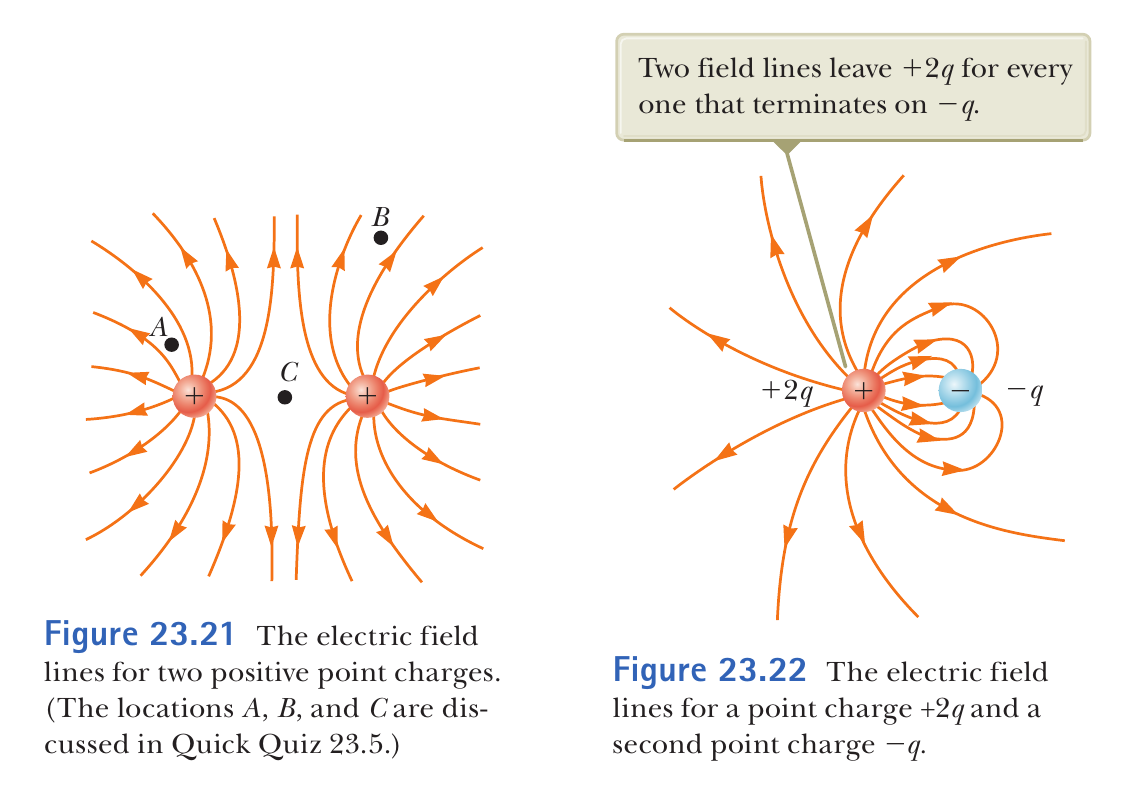
\includegraphics[scale=0.4]{3.png} Simple Parallel Circuit
		\end{center}
	
	\section*{28.3 Kirchhoff's Laws}
	\noindent\fbox{%
		\parbox{\textwidth}{%
			\begin{align}
			\sum_{Junction}i = i_{in} + i_{out} = 0
			\end{align}
			where $i_{in}$ is positive and $i_{out}$ is negative.
			\begin{align}
			\sum_{Closed \hspace{1mm} loop} \Delta V = 0
			\end{align}
			while following passive sign convention.
		}}
	\end{document}